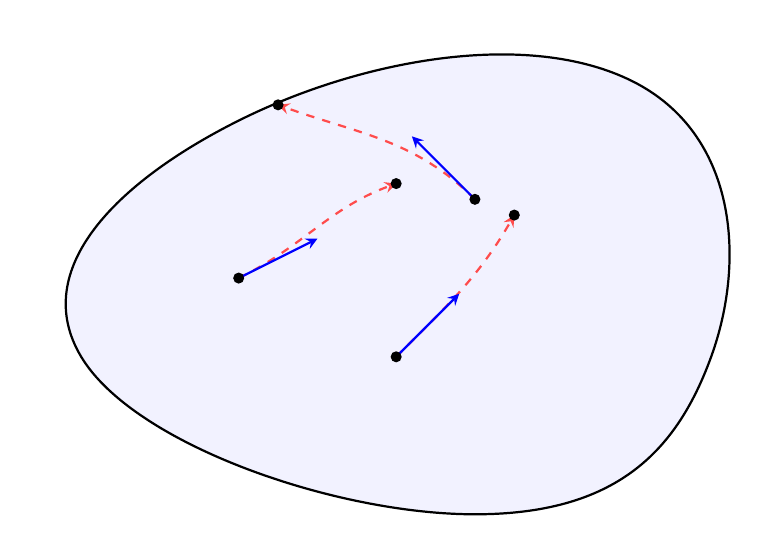
\begin{tikzpicture}[>=stealth]
    % 1. Draw the Manifold
    % Using a smooth cycle to create an organic, topological shape
    \draw[thick, fill=blue!5] plot [smooth cycle, tension=0.8] coordinates {
            (-2,-1) (0,2) (5,2.5) (6,-1) (3,-3)
        };
    \node[scale=1.5, black!100] at (4.5,-2) {};

    % 2. Define coordinates for the points (q_i)
    \coordinate (q1) at (0,0);
    \coordinate (q2) at (2,-1);
    \coordinate (q3) at (3,1);

    % 3. Define the vectors X(q_i)
    % The vector tips are placed relative to the starting points
    \coordinate (vq1) at (1, 0.5); % Angle ~ 26 degrees
    \coordinate (vq2) at (2.8, -0.2); % Angle = 45 degrees
    \coordinate (vq3) at (2.2, 1.8); % Angle = 135 degrees

    % 4. Define the flowed points \varphi_t(q_i)
    \coordinate (phi1) at (2, 1.2);
    \coordinate (phi2) at (3.5, 0.8);
    \coordinate (phi3) at (0.5, 2.2);

    % 5. Draw the flow lines (Trajectories)
    % The 'out' angle matches the tangent of the vector field at that point
    \draw[->, dashed, thick, red!70] (q1) to[out=26, in=200] (phi1);
    \draw[->, dashed, thick, red!70] (q2) to[out=45, in=240] (phi2);
    \draw[->, dashed, thick, red!70] (q3) to[out=135, in=340] (phi3);

    % 6. Draw the vectors
    \draw[->, thick, blue] (q1) -- (vq1) node[midway, below right] {};
    \draw[->, thick, blue] (q2) -- (vq2) node[midway, below right] {};
    \draw[->, thick, blue] (q3) -- (vq3) node[midway, above right] {};

    % 7. Draw and label the points
    \fill[black] (q1) circle (2pt) node[left] {};
    \fill[black] (q2) circle (2pt) node[left] {};
    \fill[black] (q3) circle (2pt) node[right] {};

    \fill[black] (phi1) circle (2pt) node[right] {};
    \fill[black] (phi2) circle (2pt) node[right] {};
    \fill[black] (phi3) circle (2pt) node[left] {};

\end{tikzpicture}